%=====================================================
\begin{frame}{3.1.2. Декларируемый уровень доверия к руководству (группы по возрасту) }

\tiny

На диаграмме представлен результат по вопросу Б18 с разбивкой по возрасту:
\bigskip

\centering 

\begin{tabular}{|l|c|c|c|c|} \hline
& до 25 лет &  25 -- 35  лет &  36 -- 55 лет & свыше 55 лет \\ \hline
Ответили утвердительно & & & & \\
(``да'' или ``скорее да, чем нет'')  & \valCAByesNumA     &   \valCAByesNumB         &   \valCAByesNumC  & \valCAByesNumD \\ \hline
Ответили отрицательно  & & & & \\
(``нет'' или ``скорее нет, чем да'') & \valCABnoNumA  &  \valCABnoNumB    &   \valCABnoNumC   & \valCABnoNumD  \\ \hline
\end{tabular}
\bigskip

\begin{tabular}{cccc}
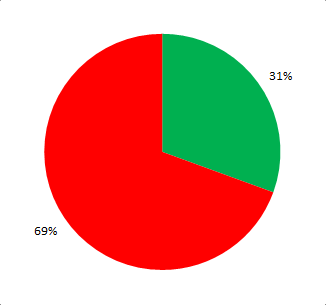
\includegraphics[width=2.2cm, height=2.2cm]{diag.png} & 
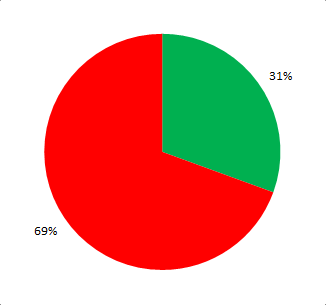
\includegraphics[width=2.2cm, height=2.2cm]{diag.png} & 
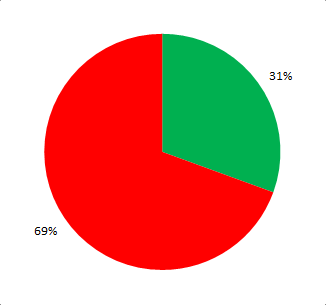
\includegraphics[width=2.2cm, height=2.2cm]{diag.png} & 
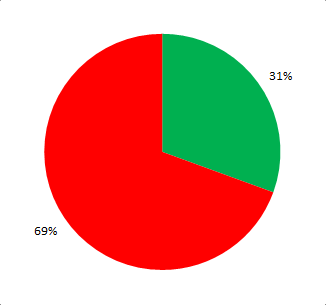
\includegraphics[width=2.2cm, height=2.2cm]{diag.png} \\
до 25 лет &  25 -- 35  лет &  36 -- 55 лет & свыше 55 лет \\
\end{tabular}

\end{frame}


